\documentclass[oneside,senior,etd]{BYUPhysForDegree}

\usepackage[utf8]{inputenc}
\usepackage{rotating} 

\usepackage[russian]{babel}
\usepackage{amsfonts} % Пакеты для математических символов и теорем
\usepackage{amstext}
\usepackage{amssymb}
\usepackage{amsthm}
\usepackage{graphicx} % Пакеты для вставки графики
\usepackage{subfig}
\usepackage{color}
\usepackage[unicode]{hyperref}
\usepackage[nottoc]{tocbibind} % Для того, чтобы список литературы отображался в оглавлении
\usepackage{algorithmic} % Для записи алгоритмов в псевдокоде
\usepackage{algorithm}
\usepackage{verbatim} % Для вставок заранее подготовленного текста в режиме as-is
\usepackage{listings}

\usepackage{diagbox}

\usepackage{commath}
\newcommand\Tau{\mathcal{T}}
\newcommand{\R}{\mathbb{R}}
\usepackage{color}
\usepackage[colorinlistoftodos, prependcaption]{todonotes}
\usepackage{multirow}
\newcommand*{\MyIndent}{\hspace*{0.2cm}}%


\Chair{Кафедра системного программирования}
\Lab{~}
\Year{2024}
  \Month{Февраль}
  \City{Москва}
  \AuthorText{Автор}
  \Author{Морозов Илья Федорович}
  \AuthorEng{Morozov Ilia Fedorovich}
  \AcadGroup{328}
  \TitleTop{Отчёт №1}
  % \TitleTop{JavaPrac}
  % \TitleBottom{с помощью языковых моделей}
  %\TitleMiddle{}
  % \docname{Отчёт № 1}
  
%%%% DON'T change this. It is here because .sty does not support cyrillic cp properly %%%%
\University{Московский государственный университет имени М.В.Ломоносова}
\Faculty{Факультет вычислительной математики и кибернетики}
\GrText{гр. 328}

% КОНЕЦ ТИТУЛЬНОГО ЛИСТА

\begin{document}
\fixmargins
\makepreliminarypages
\oneandhalfspace
     
 
\newpage
\section{Описание}

Пользователь, заходя на сайт, проходит обязательную аутентификацию или же регистрацию, если ранее она не была пройдена, посредством нажатия на кнопку <<Вход>> или <<Регистрация>>, соответственно. Появляется всплывающая поверх сайта форма, требующая заполнения данных для входа. При аутентификации, в случае неверного ввода выводится текст, сигнализирующий об этом. Далее ожидается повторное заполнение формы. В случае верного окно исчезает и заместо кнопок <<Вход>>, <<Регистрация>> появляется кнопка <<Выход>>, и пользователь, наконец получает доступ к основному функционалу сайта, а, именно, ко всем операциям для работы с биллинговой базой оператора связи.

На главной странице находится перечень возможных операций, полный список таков:
\begin{enumerate}
    \item Получение списка клиентов, в т.ч. по оказываемым услугам в заданном интервале времени, по характеристикам их счетов.
    \item Получение росписи операций по счету клиента за заданный интервал времени
    \item Регистрация договора об оказании услуги
    \item Регистрация поступлений на счет и списаний
    \item Добавление и удаление данных о клиенте, чтение и редактирование данных о нем
    \item Добавление и удаление услуги, чтение и редактирование данных о ней
\end{enumerate}

\newpage
Каждая операция представлена гиперссылкой, ведущей на соответствующую страницу, которая содержит весь необходимый интерфейс для работы с ней. При добавлении -- это поля для заполнения, при удалении -- это выбор из имеющихся записей в базе данных, при редактировании -- всё вместе, и выбор из имеющихся записей и поля для изменения в ней, соответственно. В случае некорректного использования (например, добавление уже имеющегося пользователя/услуги, невалидная дата и так далее) всплывает информационное окно с ошибкой. С каждой страницы с операцией возможно вернуться к их общему списку по кнопке <<Операции>>.

Таким образом, общая схема навигации по сайту выглядит так:

\begin{figure}[hbt!]
    \centering
    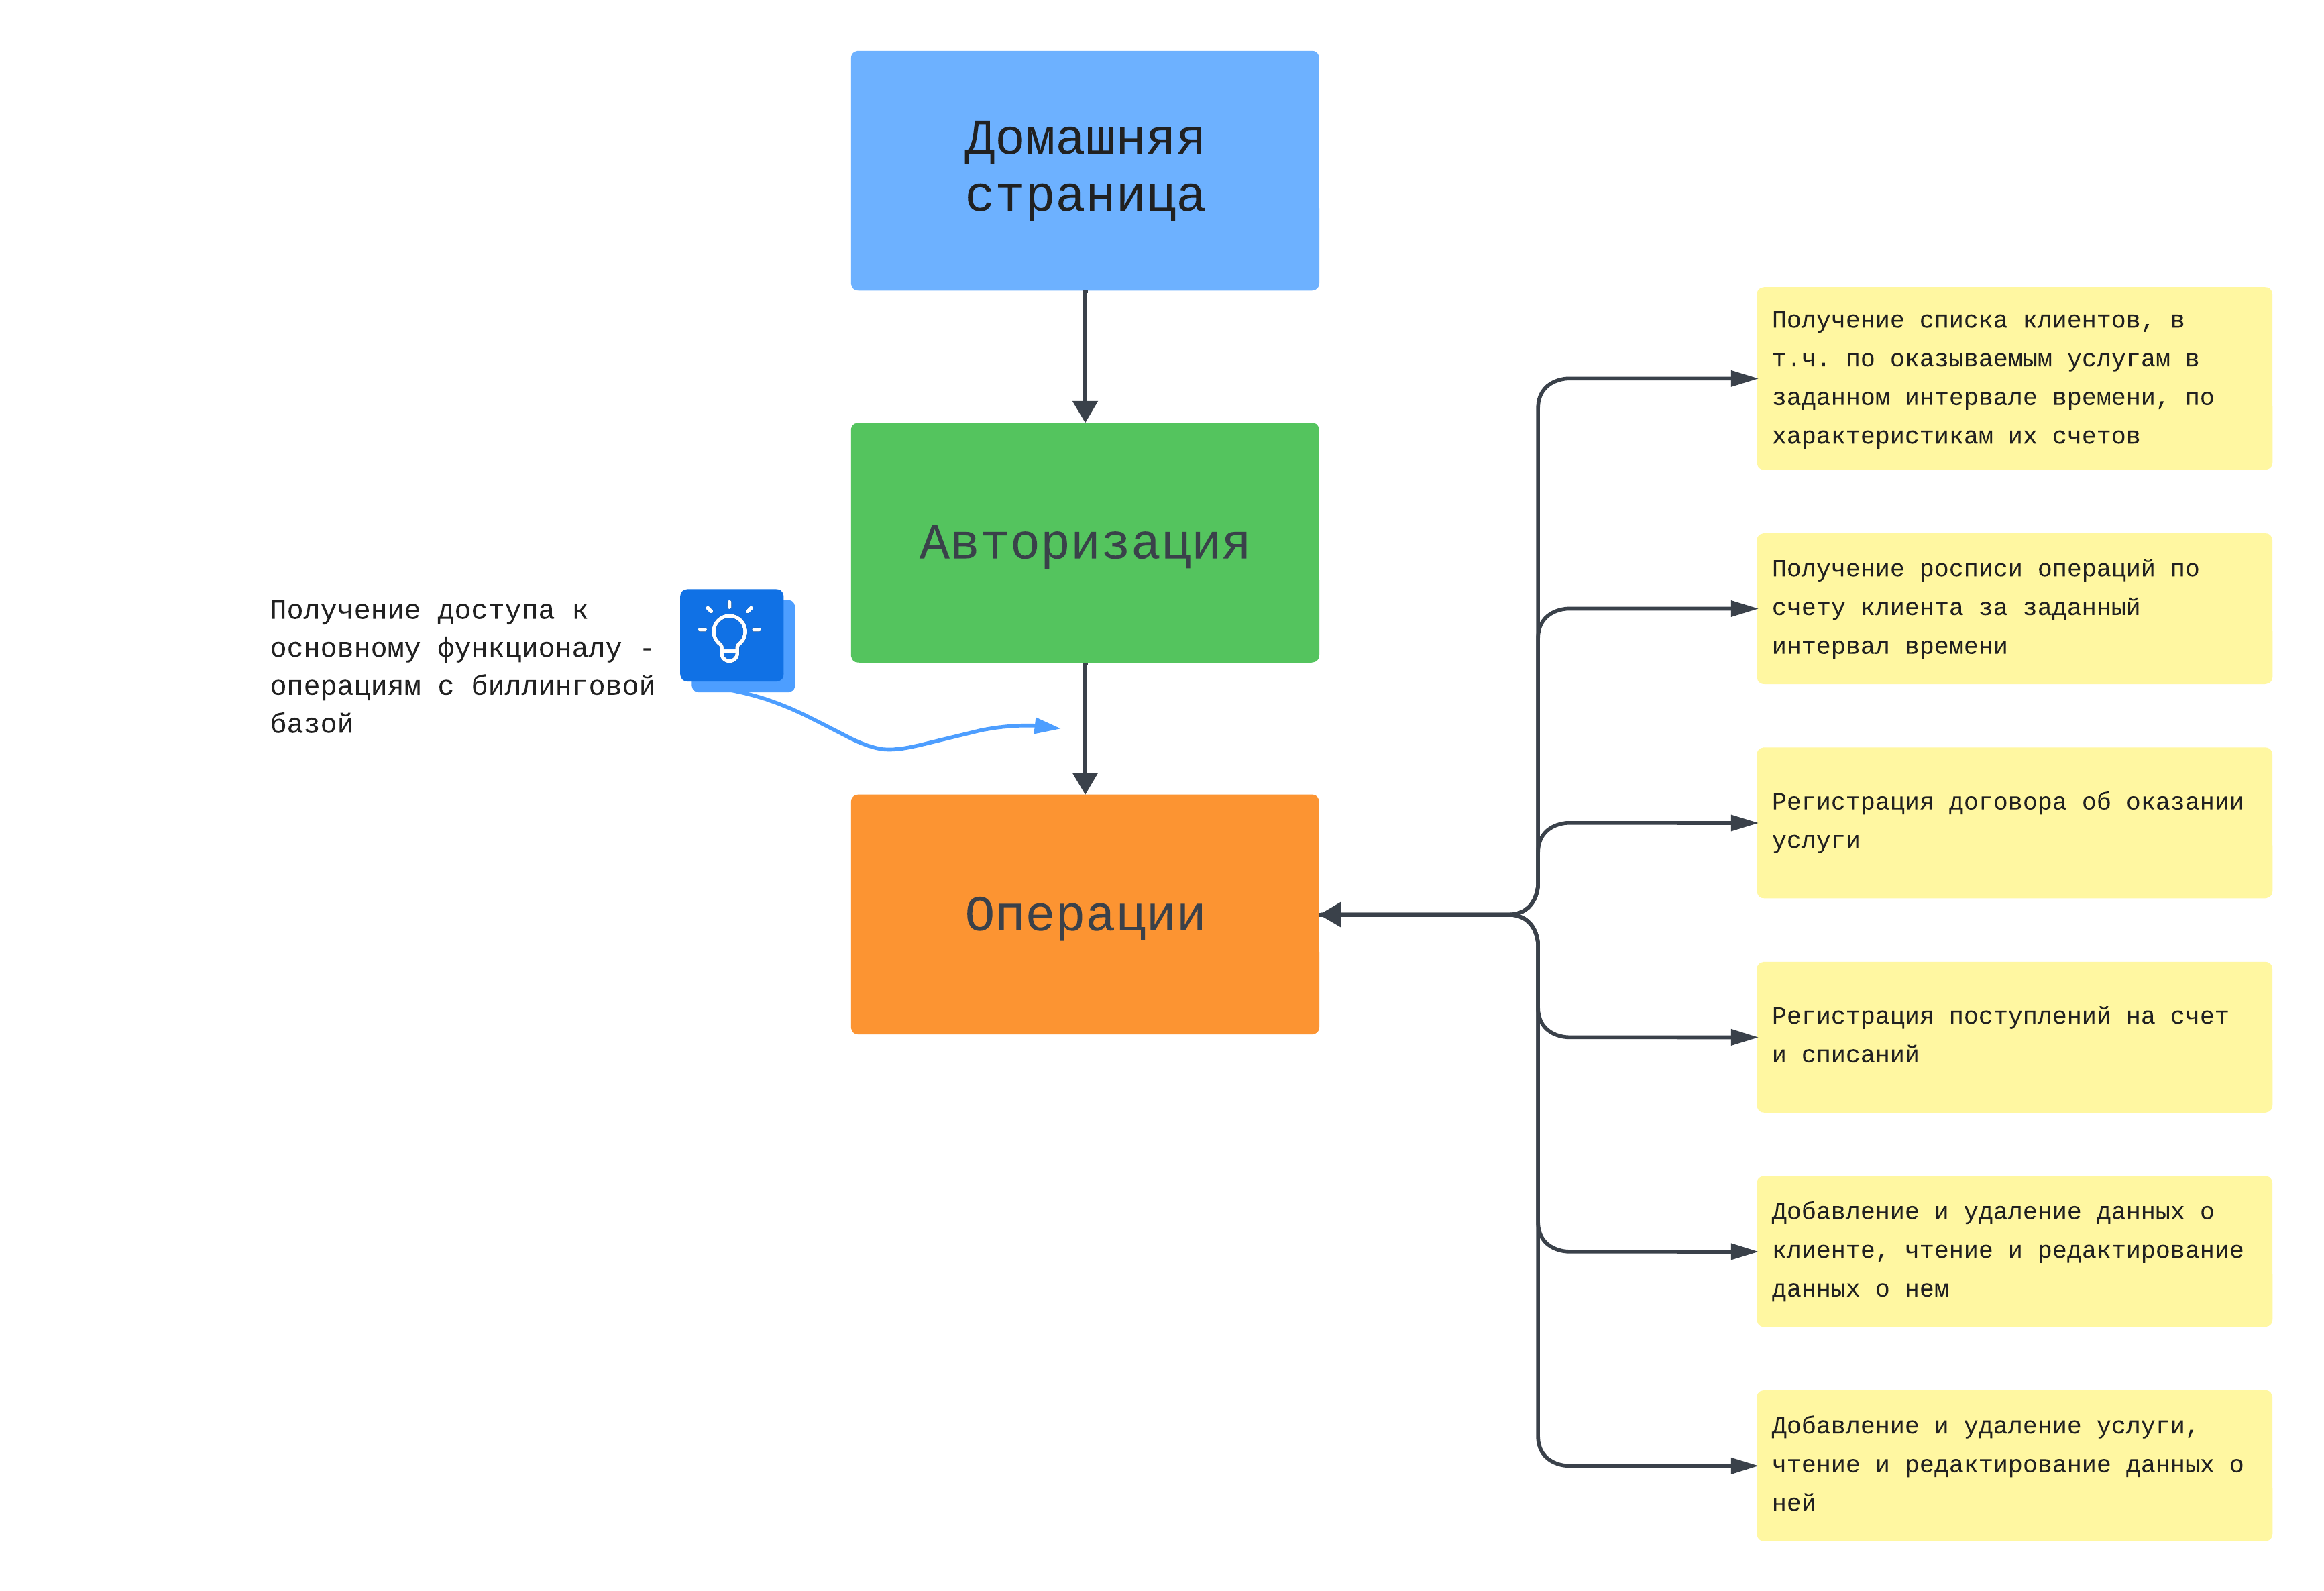
\includegraphics[width=1.0\linewidth]{sitemap.png}
    \caption{Навигация.}
    \label{fig:sitemap}
\end{figure}

\newpage
\section{База данных}

Опишем базу данных, которая будет использоваться. Ниже приведена схема, стоит дать пояснения к некоторым полям:
\begin{enumerate}
    \item acc\_history -- история поступлений и списаний по счёту в формате jsonb, где положительные числа означают приход, а отрицательные -- уход
    \item client\_contact -- список контактов с указанием телефона, адреса, email для каждого.
    \item client\_services -- перечень услуг предоставляемых пользователю в определенные промежутки времени, где услуги задаются уникальным 8-значным кодом.
    \item service\_package -- пакет, предосталяемый услугой: минуты, sms, интернет, максимальное число подключенных пользователей.
    \item service\_tariff -- цена пакета, а также тарифы минут, sms, интернета в случае исчерпания пакета.
\end{enumerate}

\begin{figure}[hbt!]
    \centering
    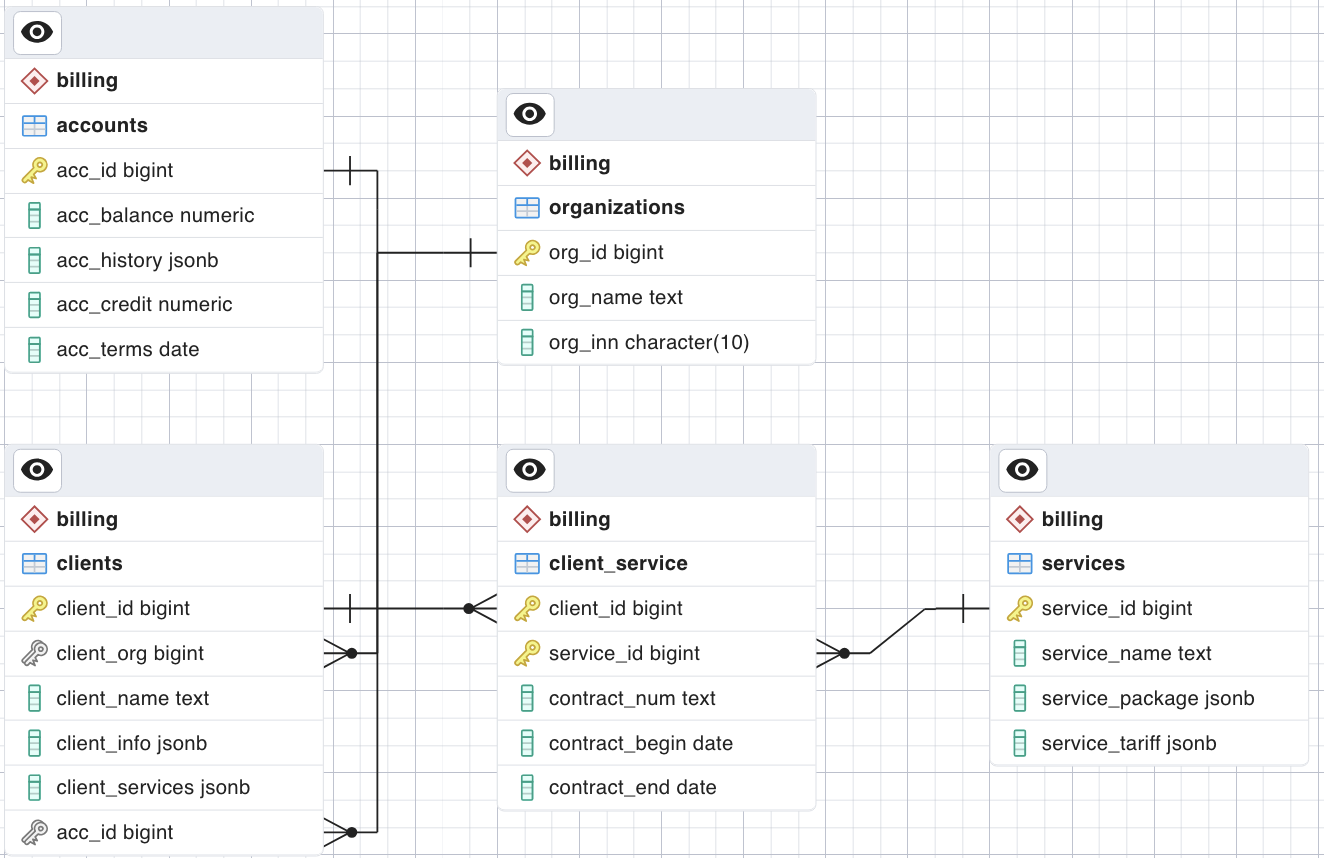
\includegraphics[width=1.0\linewidth]{scheme.png}
    \caption{Схема базы данных.}
    \label{fig:scheme}
\end{figure}



\end{document}